\documentclass[a4paper]{article}

\usepackage[T1]{fontenc}
\usepackage[utf8]{inputenc}
\usepackage{mlmodern}

%\usepackage{ngerman}	% Sprachanpassung Deutsch

\usepackage{graphicx}
\usepackage{geometry}
\geometry{a4paper, top=15mm}

\usepackage{subcaption}
\usepackage[shortlabels]{enumitem}
\usepackage{amssymb}
\usepackage{amsthm}
\usepackage{amsmath}
\usepackage{mathtools}
\usepackage{braket}
\usepackage{bbm}
\usepackage{graphicx}
\usepackage{float}
\usepackage{yhmath}
\usepackage{tikz}
\usepackage{scratch}
\usetikzlibrary{patterns,decorations.pathmorphing,positioning}
\usetikzlibrary{calc,decorations.markings}

\usepackage[backend=biber, sorting=none]{biblatex}
\addbibresource{cite.bib}

\usepackage[framemethod=TikZ]{mdframed}

\tikzstyle{titlered} =
    [draw=black, thick, fill=white,%
        text=black, rectangle,
        right, minimum height=.7cm]


\usepackage[colorlinks=true,naturalnames=true,plainpages=false,pdfpagelabels=true]{hyperref}
\usepackage[parfill]{parskip}
\usepackage{lipsum}

\usepackage{tcolorbox}
\tcbuselibrary{skins,breakable}

\pagestyle{myheadings}

\colorlet{colexam}{black}
\newcounter{definition}
\newtcolorbox[use counter=definition]{mydef}[1]{
    empty,
    title={\textbf{Definition~\thetcbcounter}~~(\textit{#1})},
    attach boxed title to top left,
    fontupper=\sl,
    boxed title style={
        empty,
        size=minimal,
        bottomrule=1pt,
        top=1pt,
        left skip=0cm,
        overlay=
            {\draw[colexam,line width=1pt]([yshift=-0.4cm]frame.north
        west)--([yshift=-0.4cm]frame.north east);}},
            coltitle=colexam,
            fonttitle=\normalfont,
            before=\par\medskip\noindent,
            parbox=false,
            boxsep=-1pt,
            left=0.75cm,
            right=3mm,
            top=4pt,
            breakable,
            pad at break*=0mm,
            vfill before first,
            overlay unbroken={
                \draw[colexam,line width=1pt]
                ([xshift=0.6cm, yshift=-0.5pt]frame.south
                west)--([xshift=0.6cm,yshift=-1pt]frame.north west)
                --([xshift=0.6cm]frame.south west)--([xshift=-13cm]frame.south east); },
            overlay first={
                \draw[colexam,line width=1pt]
                ([xshift=0.6cm, yshift=-0.5pt]frame.south
                west)--([xshift=0.6cm,yshift=-1pt]frame.north west)
                --([xshift=0.6cm]frame.south west); },
            overlay last={
                \draw[colexam,line width=1pt]
                ([xshift=0.6cm, yshift=-0.5pt]frame.south
                west)--([xshift=0.6cm,yshift=-1pt]frame.north west)
                --([xshift=0.6cm]frame.south west)--([xshift=-13cm]frame.south east); }
}
\newcounter{theorem}
\newtcolorbox[use counter=theorem]{theorem}{
    empty,
    title={Theorem ~\thetcbcounter},
    attach boxed title to top left,
    fontupper=\sl,
    boxed title style={
        empty,
        size=minimal,
        bottomrule=1pt,
        top=1pt,
        left skip=0cm,
        overlay=
            {\draw[colexam,line width=1pt]([yshift=-0.4cm]frame.north
        west)--([yshift=-0.4cm]frame.north east);}},
            coltitle=colexam,
            fonttitle=\bfseries,
            before=\par\medskip\noindent,
            parbox=false,
            boxsep=-1pt,
            left=0.75cm,
            right=3mm,
            top=4pt,
            breakable,
            pad at break*=0mm,
            vfill before first,
            overlay unbroken={
                \draw[colexam,line width=1pt]
                ([xshift=0.6cm, yshift=-0.5pt]frame.south
                west)--([xshift=0.6cm,yshift=-1pt]frame.north west)
                --([xshift=0.6cm]frame.south west)--([xshift=-13cm]frame.south east); },
            overlay first={
                \draw[colexam,line width=1pt]
                ([xshift=0.6cm, yshift=-0.5pt]frame.south
                west)--([xshift=0.6cm,yshift=-1pt]frame.north west)
                --([xshift=0.6cm]frame.south west); },
            overlay last={
                \draw[colexam,line width=1pt]
                ([xshift=0.6cm, yshift=-0.5pt]frame.south
                west)--([xshift=0.6cm,yshift=-1pt]frame.north west)
                --([xshift=0.6cm]frame.south west)--([xshift=-13cm]frame.south east); }
}
\newcounter{lemma}
\newtcolorbox[use counter=lemma]{lemma}{
    empty,
    title={Lemma~\thetcbcounter},
    attach boxed title to top left,
    fontupper=\sl,
    boxed title style={
        empty,
        size=minimal,
        bottomrule=1pt,
        top=1pt,
        left skip=0cm,
        overlay=
            {\draw[colexam,line width=1pt]([yshift=-0.4cm]frame.north
        west)--([yshift=-0.4cm]frame.north east);}},
            coltitle=colexam,
            fonttitle=\bfseries,
            before=\par\medskip\noindent,
            parbox=false,
            boxsep=-1pt,
            left=0.75cm,
            right=3mm,
            top=4pt,
            breakable,
            pad at break*=0mm,
            vfill before first,
            overlay unbroken={
                \draw[colexam,line width=1pt]
                ([xshift=0.6cm, yshift=-0.5pt]frame.south
                west)--([xshift=0.6cm,yshift=-1pt]frame.north west)
                --([xshift=0.6cm]frame.south west)--([xshift=-13cm]frame.south east); },
            overlay first={
                \draw[colexam,line width=1pt]
                ([xshift=0.6cm, yshift=-0.5pt]frame.south
                west)--([xshift=0.6cm,yshift=-1pt]frame.north west)
                --([xshift=0.6cm]frame.south west); },
            overlay last={
                \draw[colexam,line width=1pt]
                ([xshift=0.6cm, yshift=-0.5pt]frame.south
                west)--([xshift=0.6cm,yshift=-1pt]frame.north west)
                --([xshift=0.6cm]frame.south west)--([xshift=-13cm]frame.south east); }
}

\newcommand{\eps}{\varepsilon}
\usepackage[OT2,T1]{fontenc}
\DeclareSymbolFont{cyrletters}{OT2}{wncyr}{m}{n}
\DeclareMathSymbol{\Sha}{\mathalpha}{cyrletters}{"58}

\markright{Popović\hfill Seminar\hfill}


\title{University of Vienna\\
\vspace{1cm}Seminar:\\Joint RICAM Seminar\\
\vspace{0.5cm}
Summary of talk by Otmar Scherzer
}
\author{Milutin Popovic}


\begin{document}

\maketitle
\tableofcontents

\section{Governing Equations of Fluid Dynamics}
We first start of with a fluid with a density
\begin{align}
    \rho(\mathbf{x}, t),
\end{align}
in three dimensional Cartesian coordinates $\mathbf{x} = (x, y, z)$ at time
$t$. For water-wave applications, we should note that we take
$\rho=\text{constant}$, but we will go into this fact later. The fluid moves
in time and space with a velocity field
\begin{align}
    \mathbf{u}(\mathbf{x}, t) = (u, v, w).
\end{align}
Additionally it is also described by its pressure
\begin{align}
    P(\mathbf{x}, t),
\end{align}
generally depending on time and position. When thinking of e.g. water the
pressure increases the deeper we go, that is with decreasing or increasing $z$
direction (depending how we set up our system $z$ pointing up or down
respectively).

The general assumption in fluid dynamics is the \textbf{Continuum
Hypothesis}, which assumes continuity of $\textbf{u}, \rho$ and $P$ in
$\mathbf{x}$ and $t$. In other words, we premise that the velocity field,
density and pressure are ''nice enough`` functions of position and time, such
that we can do all the differential operations we desire in the framework of
differential analysis.
\subsection{Mass Conservation}
Our aim is to derive a model of the fluid and its dynamics, with respect to
time and position, in the most general way. This is usually done thinking
of the density of a given fluid, which is a unit mass per unit volume,
intrinsically  an integral representation to derive these equations suggests
by itself.

Let us now thing of an arbitrary fluid. Within this fluid we define a fixed
volume $V$ relative to a chosen inertial frame and bound it by a surface $S$
within the fluid, such that the fluid motion $\mathbf{u}(\mathbf{x}, t)$ may
cross the surface $S$. The fluid density is given by $\rho(\mathbf{x}, t)$,
thereby the mass of the fluid in the defined Volume $V$ is an integral
expression
\begin{align}
    m = \int_V \rho(\mathbf{x}, t) dV.
\end{align}
The figure bellow \ref{fig:volume}, expresses the above described picture.
\begin{figure}[H]
    \centering
  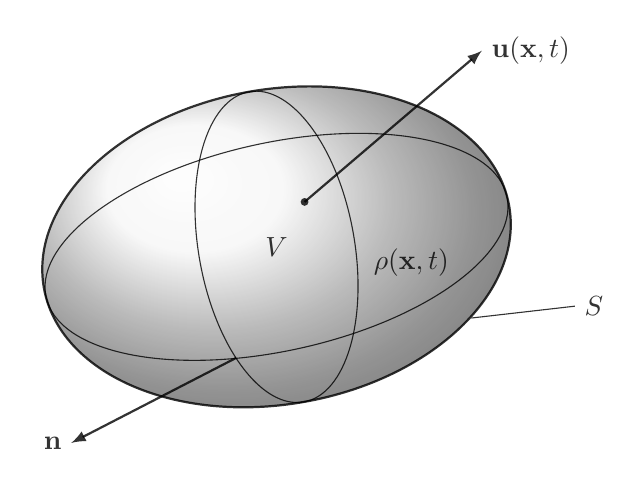
\begin{tikzpicture}[>=latex,scale=1, xscale=1, opacity=.8]
% second sphere
    \begin{scope}[rotate=10, xscale=3, yscale=2, shift={(2.3,-0.2)}]
      \coordinate (O) at (0,0);
      \shade[ball color=gray!10!] (0,0) coordinate(Hp) circle (1) ;

      \draw[thick] (O) circle (1);
      \draw[rotate=5] (O) ellipse (1cm and 0.66cm);
      \draw[rotate=90] (O) ellipse (1cm and 0.33cm);
\node[circle, fill=black, inner sep=1pt] at (0.15, 0.25) {} ; \draw[-latex, thick] (0.15, 0.25) -- (1, 1) ;
      \node[right] at (1, 1) {$\mathbf{u}(\mathbf{x}, t)$};

      \node[] at (O) {$V$};
      \node[] at (0.55, -0.25) {$\rho(\mathbf{x}, t)$};

      \draw[-] (0.76, -0.66) -- (1.2, -0.7);
      \node[right] at (1.2, -0.7) {$S$};

      \draw[-latex, thick] (-0.25, -0.65) -- (-1, -1);
      \node[left] at (-1, -1) {$\mathbf{n}$};

    \end{scope}

% axis
  \end{tikzpicture}
  \caption{Volume bounded by a surface in a fluid with density and momentum,
  with a surface normal vector $\mathbf{n}$ \label{fig:volume}}
\end{figure}

Since we want to figure out the fluid's dynamics, we can consider the rate
of change in the completely arbitrary $V$. The rate of change of mass needs to
disappear, i.e. it is equal to zero since we cannot lose mass. Matter (mass) is
neither created nor destroyed anywhere in the fluid, leading us to
\begin{align}
    \frac{d}{dt}\left( \int_V \rho(\mathbf{x}, t)\ dV \right) = 0.
\end{align}
To get more information we simply ''differentiate under the integral
sign``, also known as the Leibniz Rule of Integration, see appendix
\ref{appendix:leibniz}, the integral equation representing the rate of change
of mass reads
\begin{align}\label{eq:mass balance}
    \frac{dm}{dt} = \int_V \frac{\partial \rho(\mathbf{x}, t)}{\partial t}\ dV
    +\int_{\partial V} \rho(\mathbf{x}, t) \mathbf{u}\cdot\mathbf{n}\ dS
    = 0.
\end{align}
The above equation in \ref{eq:mass balance} is an underlying equation, describing that the rate of
change of mass in V is brought about, only by the rate of mass flowing into
V across S, and thus the mass does not change.

For the second integral in \ref{eq:mass balance} we utilize the Gaussian
integration law to acquire an integral over the volume
\begin{align}
    \int_{\partial V} \rho(\mathbf{x}, t) \mathbf{u} \cdot \mathbf{n} \ dS =
    \int_V \nabla (\rho \mathbf{u})\ dV.
\end{align}
Thereby we can put everything inside the volume integral
\begin{align}
    \frac{d m}{dt} = \int_V \left(\partial_t \rho + \nabla(\rho \mathbf{u}) \right) \ dV = 0.
\end{align}
Everything under the integral sign needs to be zero, thus we obtain
the \textbf{Equation of Mass Conservation} or in the general sense also
called the \textbf{Continuity Equation}
\begin{align}\label{eq:continuity}
    \partial_t \rho + \nabla(\rho \mathbf{u}) = 0
\end{align}

In light of the results of the equation of mass conservation
in \ref{eq:continuity}, an product rule gives
\begin{align}
    \partial_t \rho + (\nabla \rho)\mathbf{u} + \rho(\nabla \mathbf{u}),
\end{align}
for notational purposes, we define the \textbf{material/convective derivative}
as follows
\begin{align}
    \frac{D}{Dt} = \partial_t + \mathbf{u}\nabla.
\end{align}
With the material derivative the equation of mass conservation reads
\begin{align}
    \frac{D\rho}{Dt} + \rho \nabla\mathbf{u} = 0
\end{align}
We may undertake the first case separation, initiating $\rho = \text{cosnt.}$
called \textbf{incompressible flow} causes the material derivative of $\rho$ to
be zero, and thereby
\begin{align}
    \frac{D\rho}{Dt} = 0 \quad \Rightarrow \quad \nabla \mathbf{u} = 0,
\end{align}
following that the divergence of the velocity field is zero, in this case
$\mathbf{u}$ is called \textbf{solenoidal}.
\subsection{Euler's Equation of Motion}
Additional consideration we undertake is the assumption of an
\textbf{inviscid} fluid, that is we set viscosity to zero. Otherwise we would
get a viscous contribution under the integral which results in the
Navier-Stokes equation. In this regard we apply Newton's second law to our
fluid in terms of infinitesimal pieces $\delta V$ of the fluid. The
acceleration divides into two terms, a \textbf{body force} given by gravity
of earth in the $z$ coordinate $\mathbf{F} = (0, 0, -g)$ and a
\textbf{local/short-rage force} described by the stress tensor in the fluid.
In the inviscid case we the local force retains the pressure $P$, producing a
normal force, with respect to the surface, acting onto any infinitesimal
element in the fluid. The integral formulation of the force would be
\begin{align}
    \int_V \rho \mathbf{F}\ dV - \int_S P\mathbf{n}\ dV.
\end{align}
Now applying the Gaussian rule of integration on the second integral over the
surface, the resulting force in per unit volume is
\begin{align}
    \int_V \left(\rho \mathbf{F} - \nabla P\right)\ dV.
\end{align}
The acceleration of the fluid particles is given by $\frac{D\mathbf{u}}{Dt}$,
and thus the total force per unit volume on the other hand is
\begin{align}
    \int_V \rho \frac{D\mathbf{u}}{Dt}\ dV =
    \int_V \left(\rho \mathbf{F} - \nabla P\right)\ dV.
\end{align}
Newton's Second Law for a fluid in an Volume is essentially saying that the
rate of change of momentum of the fluid in the fixed volume $V$, which is the particle
acceleration is the resulting force acting on V together with the rate of
flow of momentum across the surface $S$ into the volume $V$. Hence we arrive
at the \textbf{Euler's Equation(s) of Motion}
\begin{align}
    \frac{D\mathbf{u}}{Dt} = \left(\frac{\partial \mathbf{u}}{\partial t}
    (\mathbf{u}\nabla)\mathbf{u}\right)  =
    -\frac{1}{\rho}\nabla P + \mathbf{F}.
\end{align}
As a side note we have mentioned that there is another contribution if the
fluid is viscid. Indeed there is a tangential force due to the velocity
gradient, which into introduces the additional term
\begin{align}
    \mu \nabla^2 \mathbf{u}, \qquad
    \mu = \text{viscosity of the Fluid}.
\end{align}
Thereby the equations become
\begin{align}
    \rho\frac{D\mathbf{u}}{Dt}
    =  -\nabla P + \rho \mathbf{F} + \mu \nabla^2 \mathbf{u}.
\end{align}

For now we have separated two simplifications, that define an
\textbf{idealized/perfect fluid}
\begin{enumerate}
    \item \textbf{incompressible} $\qquad \mu=0$
    \item  \textbf{inviscid} $\quad \rho = \text{const.},\ \nabla \mathbf{u}=
        0$
\end{enumerate}
\subsection{Vorticity and irrotational Flow}
The curl of the velocity field $\mathbf{\omega} = \nabla \times \mathbf{u}$
of a fluid (i.e. the vorticity), describes a spinning motion of the fluid
near a position $\mathbf{x}$ at time $t$. The vorticity is an important
property of a fluid, flows or regions of flows where $\mathbf{\omega}=0$ are
\textbf{irrotational}, and thus can be modeled and analyzed following well
known routine methods. Even though real flows are rarely irrotational
anywhere (!), in water wave theory wave problems, from the classical aspect
of vorticity have a minor contribution. Hence we can assume irrotational flow
modeling water waves. To arrive at the vorticity in the equations of motions
derived in the last section we resort to a differential identity derived in appendix
\ref{appendix:diff identity}, which gives for the material derivative
\begin{align}
    \frac{D\mathbf{u}}{Dt} = \frac{\partial \mathbf{u}}{\partial t}
    \nabla(\frac{1}{2}\mathbf{u}\mathbf{u)}
    - \left( \mathbf{u}\times (\nabla \times  \mathbf{u} \right).
\end{align}
Thus the equations of motion become
\begin{align}
    \frac{\partial \mathbf{u}}{\partial t} + \nabla\left(
    \frac{1}{2}\mathbf{u}\mathbf{u} + \frac{P}{\rho} + \Omega \right)
    = \mathbf{u} \times  \mathbf{\omega},
\end{align}
where $\Omega$ is the force potential per
unite mass given by $\mathbf{F} = -\nabla \Omega$.

At this point we may differentiate between \textbf{stead and unsteady flow}.
For \textbf{Steady Flow} we assume that $\mathbf{u}, P$ and $\Omega$ are time
independent, thus we get
\begin{align}
      \nabla\left( \frac{1}{2}\mathbf{u}\mathbf{u} + \frac{P}{\rho} + \Omega
      \right)  = \mathbf{u} \times  \mathbf{\omega}.
\end{align}
It is general knowledge that the gradient of a function $\nabla f$ is
perpendicular the level sets of $f(\mathbf{x})$, where $f(\mathbf{x}) =
\text{const.}$. Thus $\mathbf{u} \times  \mathbf{\omega}$ is orthogonal to
the surfaces  where
\begin{align} \label{eq:bernoulli}
    \frac{1}{2}\mathbf{u}\mathbf{u} + \frac{P}{\rho} + \Omega =
    \text{const.},
\end{align}
The above equation is called \textbf{Bernoulli's Equation}.

Secondly \textbf{Unsteady Flow} but irrotational (+ incompressible), first of
all gives us the condition for the existence of a velocity potential $\phi$
in the sense
\begin{align}
    \mathbf{\omega} = \nabla \times  \mathbf{u} = 0  \quad \Rightarrow \quad
    \mathbf{u} = \nabla \phi,
\end{align}
where $\phi$ needs to satisfy the Laplace equation
\begin{align}
    \Delta \phi = 0.
\end{align}
According to the Theorem of Schwartz we may exchange $\frac{\partial
}{\partial t}$ and $\nabla$, giving us an expression for the material
derivative
\begin{align}
    \nabla\left( \frac{\partial \phi}{\partial t} +\frac{1}{2}
    \mathbf{u}\mathbf{u} + \frac{P}{\rho}  + \Omega \right) = 0
\end{align}
Thus the expression differentiated by the $\nabla$ operator is an arbitrary
function $f(\mathbf{x}, t)$, writing
\begin{align}
     \frac{\partial \phi}{\partial t} +\frac{1}{2}
    \mathbf{u}\mathbf{u} + \frac{P}{\rho}  + \Omega = f(\mathbf{x}, t).
\end{align}
The function $f(\mathbf{x}, t)$ can be removed by gauge transformation of
$\phi \rightarrow \phi + \int f(\mathbf{x}, t)\ dt$, never the less this is
not further discussed and left to the reader in the reference.
\subsection{Boundary Conditions for water waves}
Surface, Bottom, Pressure




\newpage
\appendix
\section{Appendix: Mathematical Preliminaries}
\subsection{Leibniz Rule of Integration}
\label{appendix:leibniz}
The Leibniz integral rule for differentiation under the integral sign
initiates with an integral
\begin{align}
    \mathcal{I}(t, x) = \int_{a(t)}^{b(t)} f(t, x) dx = \mathcal{I}(t, a(t,
    a(t), b(t))).
\end{align}
And upon differentiation w.r.t. $t$, utilizes the chain rule on $a(t)$ and
$b(t)$ respectively, by
\begin{align}
    \frac{d\mathcal{I}}{dt} =
    \frac{\partial \mathcal{I}}{\partial t}+
    \frac{\partial \mathcal{I}}{\partial a}\frac{\partial a}{\partial t}+
    \frac{\partial \mathcal{I}}{\partial b}\frac{\partial b}{\partial t}.
\end{align}
Which in integral representation reads
\begin{align}
    \frac{d\mathcal{I}}{dt} = \int_{a(t)}^{b(t)}\frac{\partial f(t,
    x)}{\partial t} dx + f(t, b(t)) \frac{\partial b(t)}{\partial t}
    - f(t, a(t)) \frac{\partial a(t)}{\partial t}
\end{align}

\subsection{Identity for Vorticity}
\label{appendix:diff identity}
We start off with the standard material derivative
\begin{align}
    \frac{D\mathbf{u}}{Dt} = \frac{\partial \mathbf{u}}{\partial t}
    +(\mathbf{u}\nabla)\mathbf{u}.
\end{align}
We will use Einstein's Summation Convention, where we sum over indices that
both appear at as the bottom as the top index, to rewrite the second part of
the material derivative $(\mathbf{u}\nabla)\mathbf{u}$ into
\begin{align}
    (\mathbf{u}\times (\nabla \times \mathbf{u}))_k
    &= \varepsilon^{ijk}u_j(\nabla \times  \mathbf{u})_k \\
    &= \varepsilon^{ijk}u_j\varepsilon_{klm}\partial^l u^m\\
    &=(\delta^i_l\delta^j_m-\delta^i_m\delta^j_l)u_j\partial^l u^m\\
    &=u_m\partial^i u^m - u_l \partial^l u^i.\label{eq:identity split}
\end{align}
Now the first part in equation \ref{eq:identity split} can be rewritten into
\begin{align}
    u_m\partial^i u^m =\partial^i (\frac{1}{2}u_mu^m) .
\end{align}
Thus we get
\begin{align}
    (\mathbf{u}\times (\nabla \times \mathbf{u}))_k
    = \frac{1}{2}\partial^i(u_m u^m) + u_l \partial^l u^i,
\end{align}
which is
\begin{align}
    (\mathbf{u}\nabla)\mathbf{u} = \nabla(\frac{1}{2}\mathbf{u}\mathbf{u}) -
    \left(\mathbf{u}\times (\nabla \times  \mathbf{u})\right)
\end{align}
\subsection{Middle Curvature of an Implicit Function}
\label{appendix:curvature}
In our case the implicit function for fixed time reads
\begin{align}
    z-h\left(x_1,x_2\right) = 0.
\end{align}
The parametric representation is
\begin{align}
    \mathbf{\sigma} = \begin{pmatrix} x_1 \\ x_2 \\ h \end{pmatrix} .
\end{align}
The middle curvature of the surface parametrized by $\mathbf{\sigma}$ is
\begin{align}
    \frac{1}{R} = \text{Tr}(G^{-1}B),
\end{align}
where $G$ and $B$ are given by
\begin{align}
    G_{ij} = \frac{\partial \mathbf{\sigma}}{\partial x_i} \frac{\partial
    \mathbf{\sigma}}{\partial x_j}, \\
    B_{ij} = -\mathbf{N} \frac{\partial^2 \mathbf{\sigma}}{\partial
    x_i\partial x_j},
\end{align}
where $i, j = 1, 2$ and $\mathbf{N}$ is the normal, normalized surface vector given by
\begin{align}
    \mathbf{N} &= \frac{\frac{\partial \mathbf{\sigma}}{\partial x_1}\times
    \frac{\partial \mathbf{\sigma}}{\partial x_2}}{\|\frac{\partial \mathbf{\sigma}}{\partial x_1}\times
    \frac{\partial \mathbf{\sigma}}{\partial x_2}\|} \\
               &= \frac{1}{\sqrt{h_x^2 + h_y^2 +1}} \begin{pmatrix}
               -h_x\\-h_y\\1 \end{pmatrix}.
\end{align}
Thereby the matrices $B$ and $G$ are calculated to be
\begin{align}
    G = \begin{pmatrix} 1+h_x^2 & h_xh_y\\h_xh_y & 1+h_y^2 \end{pmatrix}
    \qquad
    B =\frac{1}{\sqrt{h_x^2 +h_y^2 +1} } \begin{pmatrix}h_{x x} &
    h_{yx}\\h_{x y} & h_{yy}  \end{pmatrix}.
\end{align}
The inverse of $G$ is
\begin{align}
    G^{-1}
    &= \frac{1}{\det(G)} \text{adj}(G)\\
    &= \frac{1}{h_x^2+h_y^2 +1} \begin{pmatrix}1+h_y^2 & -h_xh_y \\-h_xh_y  &
    1+h_x^2\end{pmatrix} .
\end{align}
Hence the middle curvature is given by the follwing
\begin{align}
    \frac{1}{R} &
    = \text{Tr}(G^{-1}B)\\
                &= \frac{1}{(h_x^2 + h_y^2+1)^{\frac{3}{2}}}
    \text{Tr}\begin{pmatrix} (1+h_y)^2 h_{x x} - h_x h_y h_{xy} & *\\
    * & (1+h_x^2)h_{yy}-h_xh_yh_{xy}\end{pmatrix}\\
    &=\frac{(1+h_y^2)h_{x x}+(1+h_y^2)h_{yy} -
    2h_xh_yh_{xy}}{\left( h_x^2+h_y^2+1 \right)^{\frac{3}{2}} }.
\end{align}




\nocite{johnson_1997}
\nocite{vallis_2017}
\nocite{constantin_tsunami}
\nocite{rupert_2009}
\nocite{mathe-physik}

\printbibliography

\end{document}
